\documentclass{article}

% Packages for formatting
\usepackage{parskip}
\usepackage{graphicx}
\usepackage{geometry}
\usepackage{setspace}
\usepackage{hyperref}
\hypersetup{
    colorlinks=true,
    linkcolor=blue,
    urlcolor=blue,
    pdfborderstyle={/S/U/W 1} % Underline without border
}

% Package for code listings
\usepackage{listings}
\usepackage{xcolor}

% Define colors for syntax highlighting
\definecolor{codegreen}{rgb}{0,0.6,0}
\definecolor{codegray}{rgb}{0.5,0.5,0.5}
\definecolor{codepurple}{rgb}{0.58,0,0.82}
\definecolor{backcolour}{rgb}{0.95,0.95,0.92}

% Settings for Python code
\lstset{
    backgroundcolor=\color{backcolour},   
    commentstyle=\color{codegreen},
    keywordstyle=\color{blue},
    numberstyle=\tiny\color{codegray},
    stringstyle=\color{codepurple},
    basicstyle=\ttfamily\footnotesize,
    breakatwhitespace=false,         
    breaklines=true,                 
    captionpos=b,                    
    keepspaces=true,                 
    numbers=left,                    
    numbersep=5pt,                  
    showspaces=false,                
    showstringspaces=false,
    showtabs=false,                  
    tabsize=2
}

% Set margins
\geometry{a4paper}

\usepackage{etoolbox}

% Redefine abstract environment to make it left-aligned
\renewenvironment{abstract}{%
    \small
    \begin{flushleft}%
        \textbf{\abstractname}%
        \vspace{-\baselineskip}%
        \vspace{0.25\baselineskip}%
    \end{flushleft}%
    \list{}{%
        \setlength{\leftmargin}{0.25cm}%
        \setlength{\rightmargin}{\leftmargin}%
    }%
    \item\relax
}{%
    \endlist
}

% Title
\title{Categorize Wikipedia pages}
\date{\today}

\begin{document}

\maketitle

\begin{abstract}
This project aims to gather information from Wikipedia pages and analyze its content to categorize them.
Specifically, in this project we'll use web scraping to extract data from these pages. Then, we'll employ techniques to categorize them based on their content.
\end{abstract}

\section{Introduction}
Our project focuses on extracting and analyzing data from Wikipedia pages using web scraping techniques. Moreover, we want
to categorize our pages based on their content. In order to explain our purpose, we are going to use a example.
Let's take a look at \href{https://en.wikipedia.org/wiki/Helium}{this page} in Wikipedia which is about Helium.
As you can see, it is an article about the chemical element Helium. It talks about the history and the origin of this element. Moreover, it explains its characteristics
and its applications. What we want as our objective is to explore all these text data and categorize this page in chemistry, periodic table, and element categories.

\section{Objectives}
Our main objectives are to:
\begin{itemize}
    \item Gather raw data from Wikipedia pages as HTML.
    \item Use web scraping techniques to extract relevant information and remove unused data.
    \item Apply information retrieval techniques to identify page category based on its content.
\end{itemize}

\section{Methodology}
In this section we are going to talk about tools and techniques that we need for this project.
We'll begin by fetching Wikipedia pages for analysis.
Then, we'll employ web scraping methods using Python libraries to extract data from these pages.
Finally, we'll use information retrieval techniques to determine the appropriate categories for the extracted content.

\subsection{Gathering raw data}
Since our input is a web-page address (aka URL), we need to fetch that page data by calling its address.
Now, we don't have to manually copy and paste data from websites but a scraper can perform that task for us in a couple of seconds.
In Figure~\ref{fig:webpages}, you can see the process of fetching data from web pages.

\begin{figure}[h]
    \centering
    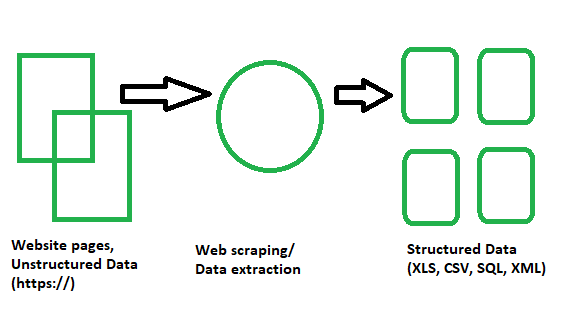
\includegraphics[width=0.5\textwidth]{./pics/web.png}
    \caption{Gathering data from webpages}
    \label{fig:webpages}
\end{figure}

As our first step, we are going to use Python \textbf{requests} library to get a web page data as HTML format.

\begin{lstlisting}[language=Python, caption=Example of getting a page content]
import requests

page = requests.get("https://en.wikipedia.org/wiki/Helium")
print(page.content)
\end{lstlisting}

In the code above, we openend a link and extracted its content as a string. Now I want you to use this example
in order to get an input link and extract its content into a string variable. Note that if the input link is incorrent, you will get
an error. Make sure to handle these types of errors by using page \underline{status code} field.

\subsection{Scraping Page Content}
Now we need to use Python beautiful soup library in order to parse HTML content in to a list of paragraphs.

\subsection{Creating Index Table}

\section{Expected Outcomes}
We anticipate achieving the following outcomes:
\begin{itemize}
    \item Successful extraction of data from Wikipedia pages using \textbf{requests} module.
    \item Accurate determination of page titles based on content analysis using \textbf{beautiful soup}.
    \item Contribution to the understanding of web scraping and information retrieval techniques.
\end{itemize}

\section{Conclusion}
In conclusion, this project aims to extract and analyze data from Wikipedia pages using web scraping and information retrieval techniques. By achieving our objectives, we hope to contribute valuable insights to the field of data analysis.

% References (if applicable)
% \bibliographystyle{plain}
% \bibliography{references}

\end{document}
